\section{Evaluation of the hybrid pipeline}\label{hybrid_pipeline_evaluation}
In this section we seek to evaluate the overall accuracy of the pipeline on the test set of \emph{Fashion-MNIST}, by 
comparing the predicted labels from the classifiers built in \Cref{hybrid_model_tuning} with the true labels. Since the labels derived 
from kernel PCA correspond to cluster IDs (which do not have any connection to the actual clothing items), a preliminary mapping step 
was necessary to enable a direct comparison between the predicted and the true labels. To perform this mapping, two procedures were considered. 
The initial approach involved associating each cluster ID with the majority label within the cluster. While straightforward, this method has
a notable limitation: the redundancy of clusters, as anticipated in \Cref{clustering} and highlighted in \Cref{fig:cluster_composition}. 
By following this approach, in fact, multiple cluster IDs would correspond to the same clothing label, resulting in certain clothing labels never 
being predicted. Notice that the latter issue arises because, by construction, the number of clusters was set equal to the number of clothing
labels. To address this limitation, I explored an alternative probabilistic mapping, where each cluster ID is assigned
to a clothing label basing on the distribution of the labels within that cluster. This method reflects the inherent uncertainty and diversity 
of the cluster composition, potentially improving labels coverage. On the other side, it introduces a non-deterministic mapping, 
which could influence negatively the overall predictive accuracy.

Classification reports are summarized in \Cref{tab:ClassificationReport_Majority,tab:ClassificationReport_Probabilistic}, while confusion matrices
are shown in \Cref{fig:confusion_matrices_majority,fig:confusion_matrices_probabilistic}.
\newpage

\begin{figure}[!htb]
    \begin{minipage}{0.33\textwidth}
      \centering
      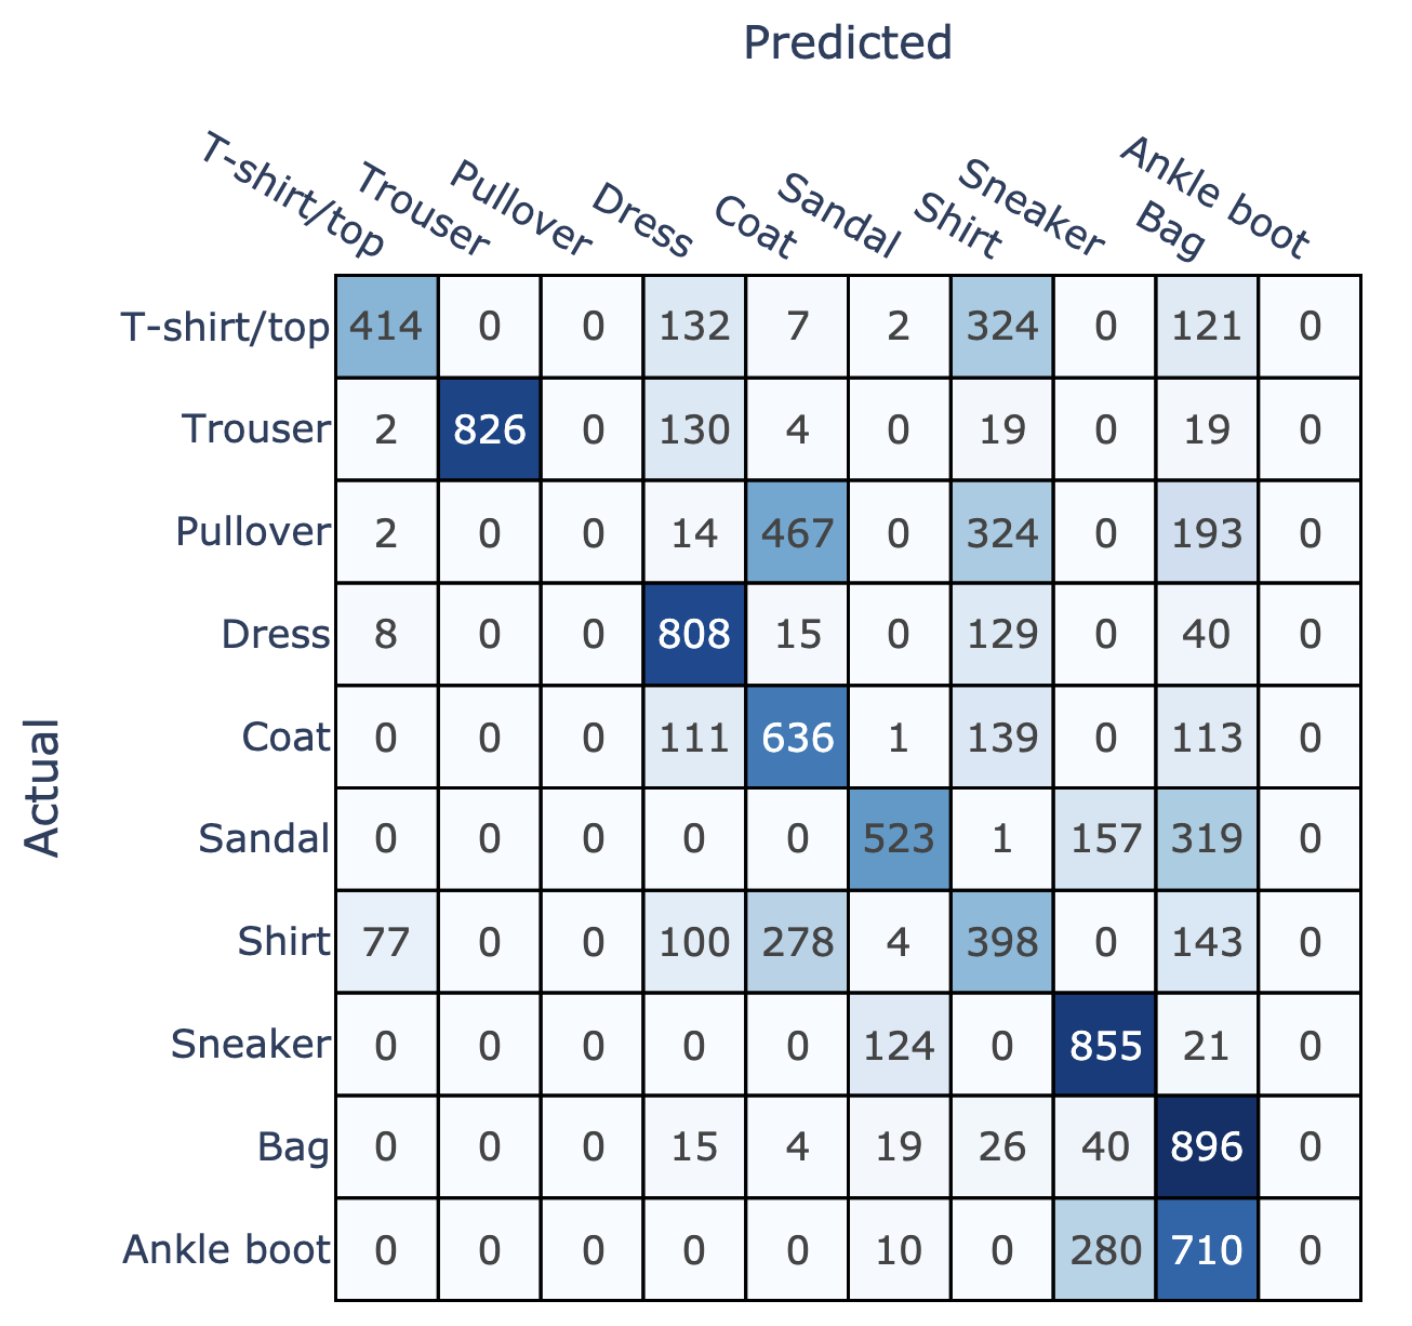
\includegraphics[width=1\linewidth]{images/CM_HybridPipeline_MajorityMapping_SVC.png}
      \subcaption{\footnotesize SVC}
    \end{minipage}\hfill
    \begin{minipage}{0.33\textwidth}
      \centering
      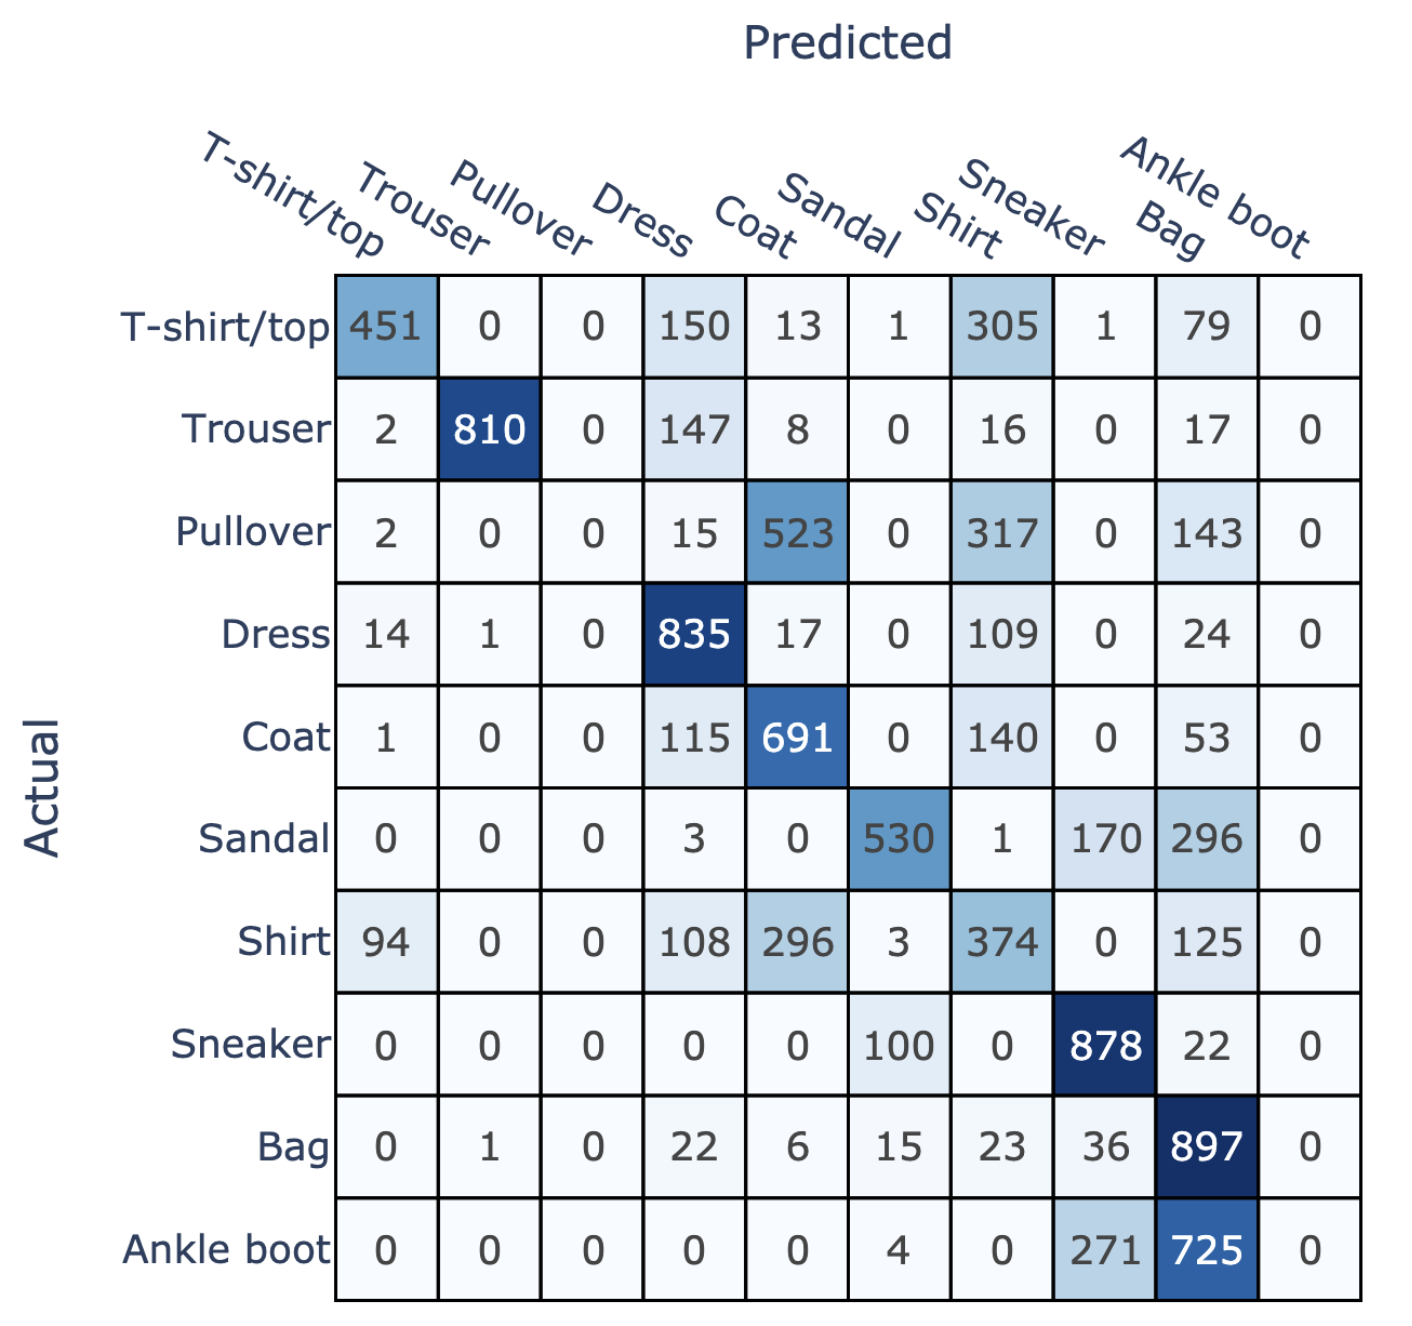
\includegraphics[width=1\linewidth]{images/CM_HybridPipeline_MajorityMapping_FCNN.png}
      \subcaption{\footnotesize FCNN}
    \end{minipage}\hfill
    \begin{minipage}{0.33\textwidth}
        \centering
        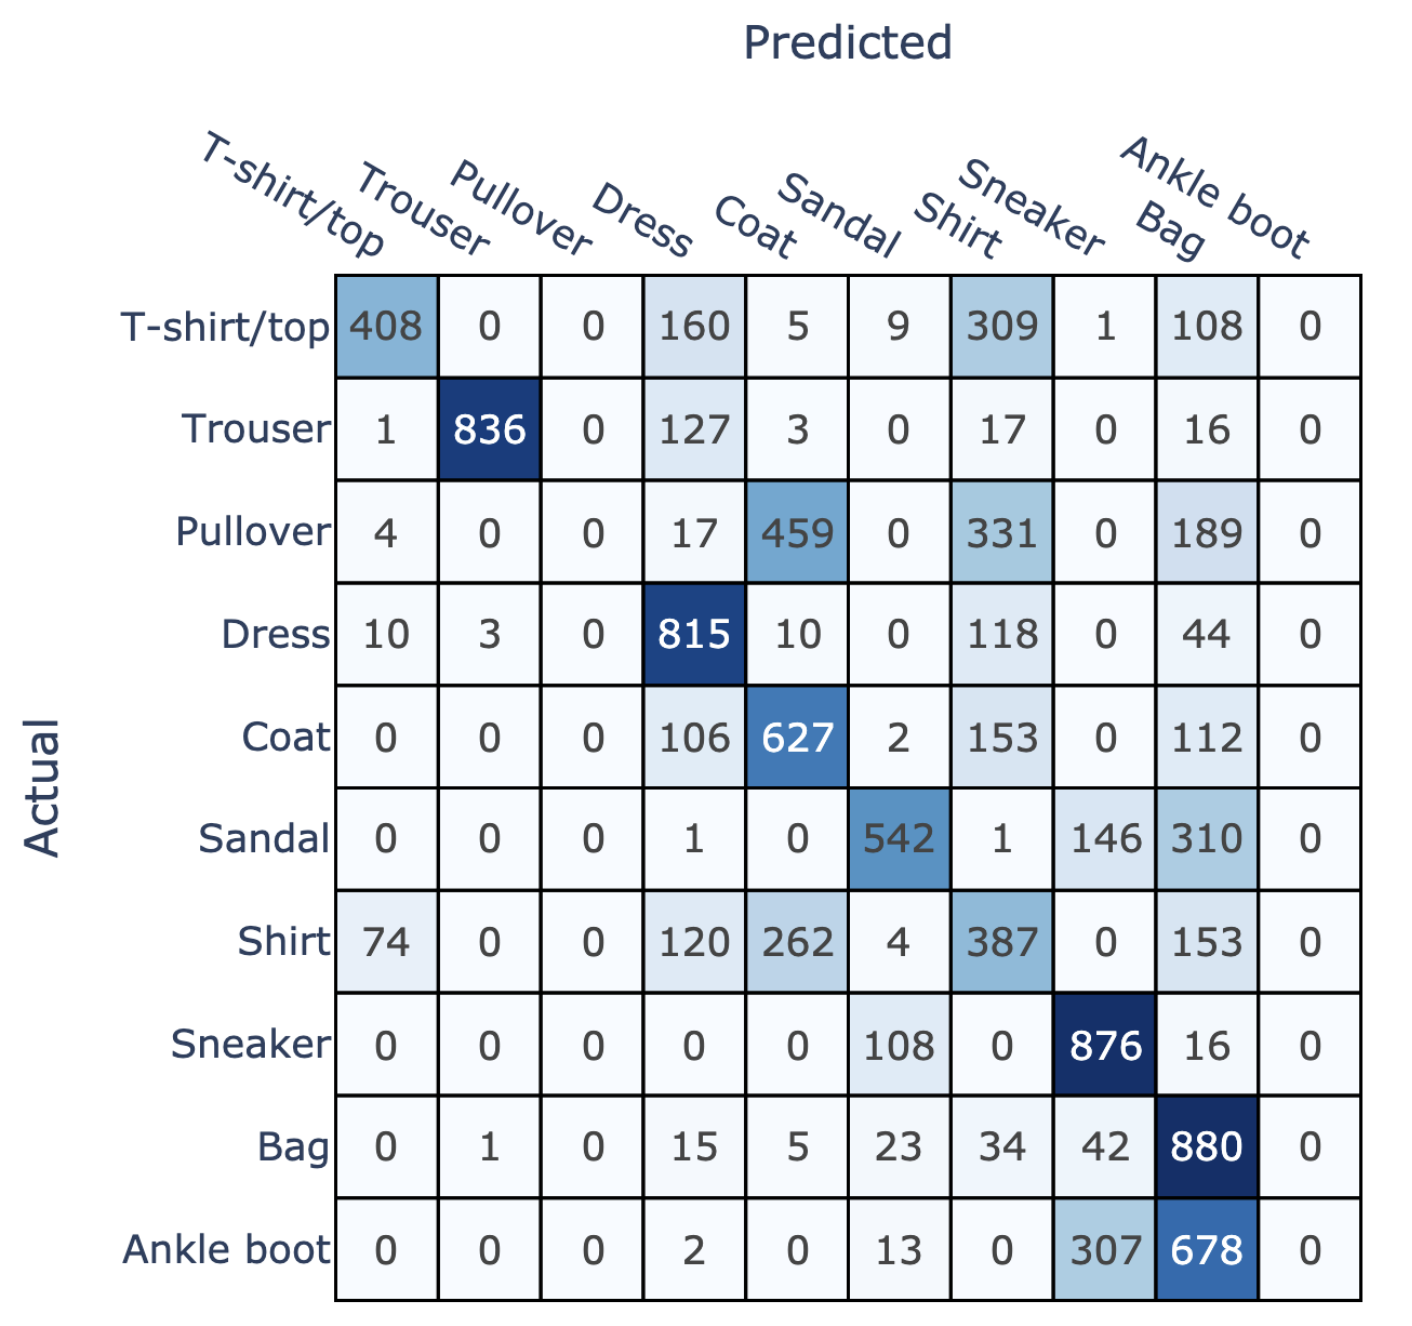
\includegraphics[width=1\linewidth]{images/CM_HybridPipeline_MajorityMapping_CNN.png}
        \subcaption{\footnotesize CNN}
    \end{minipage}
    \caption{\footnotesize Confusion matrices for classification models [Majority Mapping]}
    \label{fig:confusion_matrices_majority}
 \end{figure}

 \begin{figure}[!htb]
    \begin{minipage}{0.33\textwidth}
      \centering
      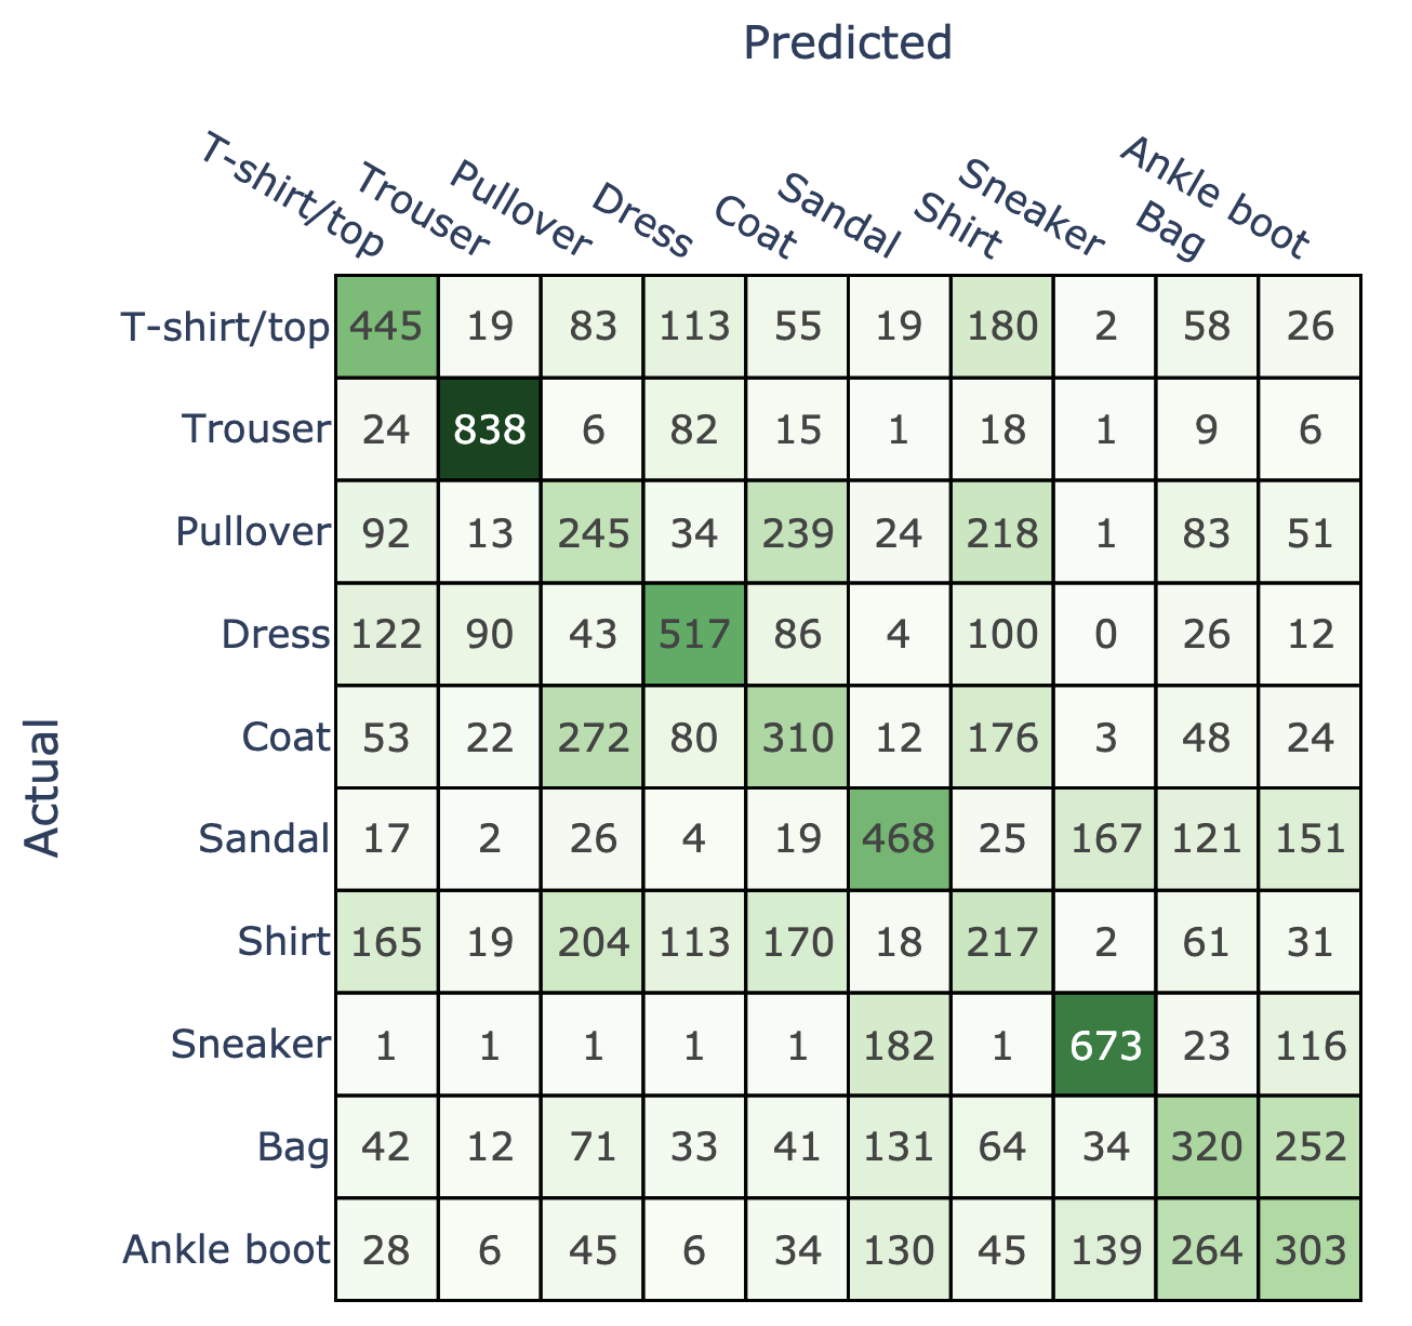
\includegraphics[width=1\linewidth]{images/CM_HybridPipeline_ProbabilisticMapping_SVC.png}
      \subcaption{\footnotesize SVC}
    \end{minipage}\hfill
    \begin{minipage}{0.33\textwidth}
      \centering
      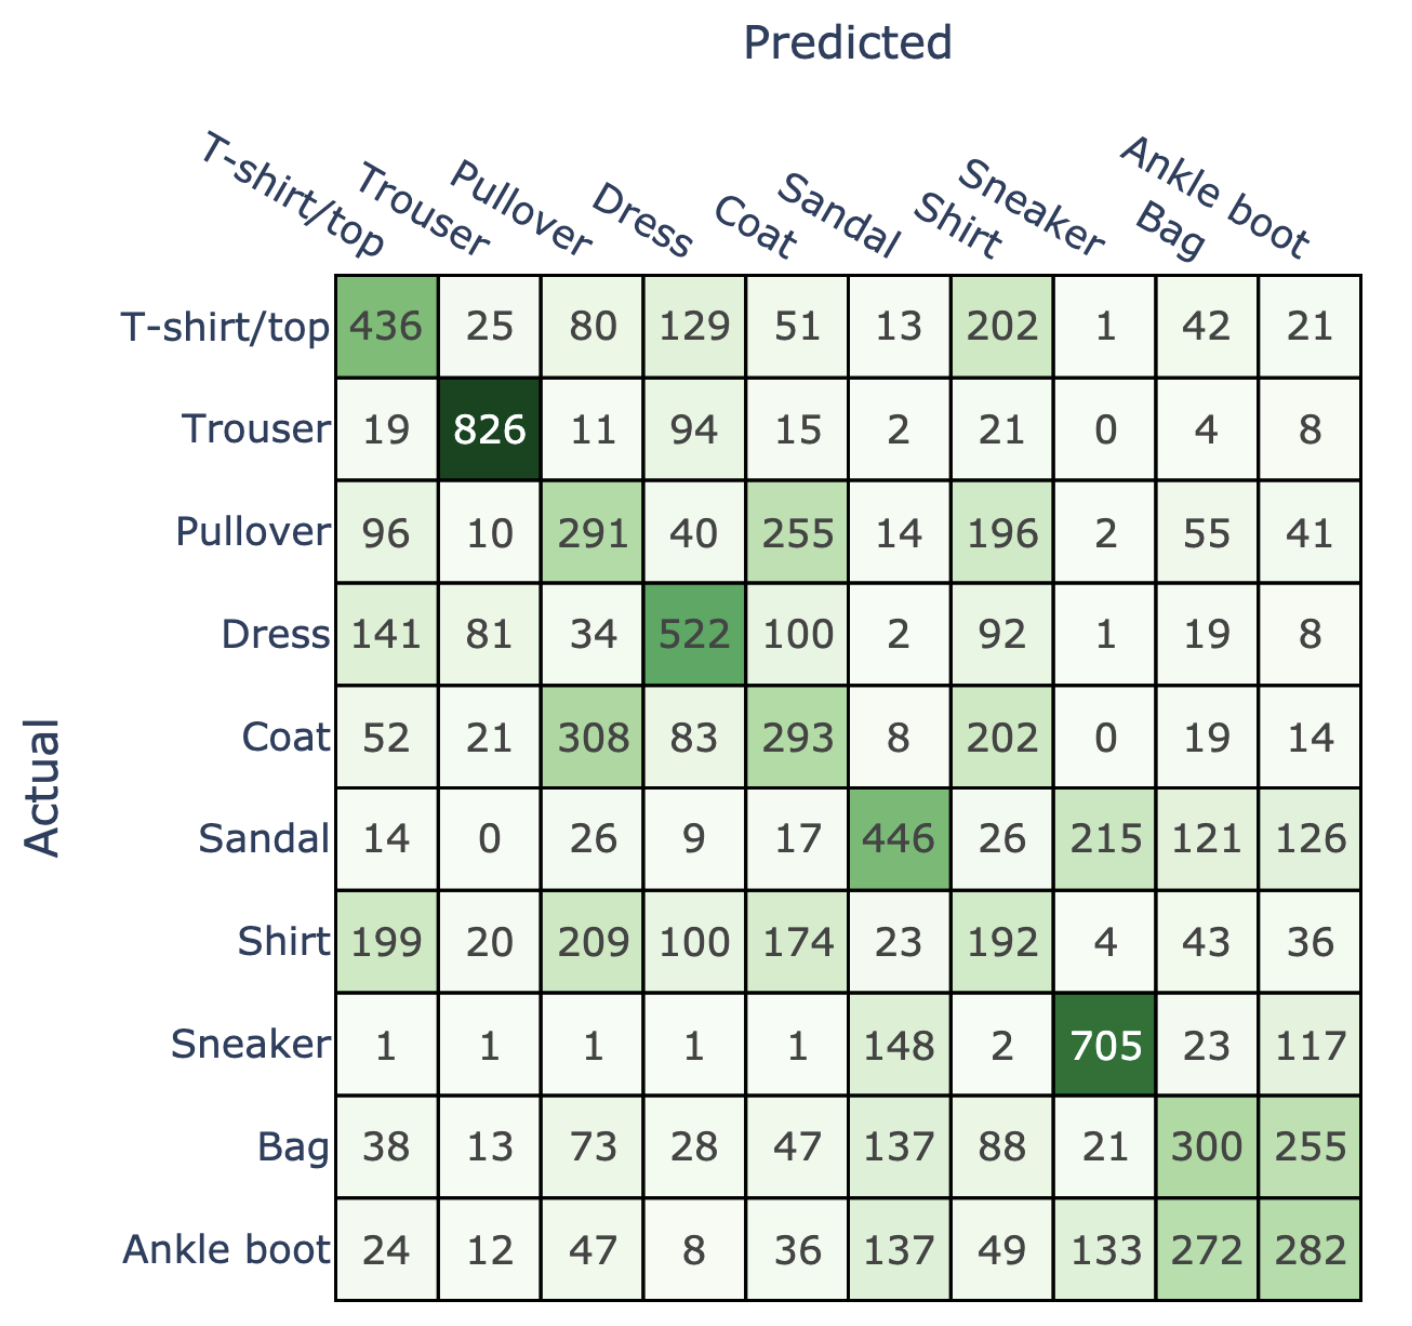
\includegraphics[width=1\linewidth]{images/CM_HybridPipeline_ProbabilisticMapping_FCNN.png}
      \subcaption{\footnotesize FCNN}
    \end{minipage}\hfill
    \begin{minipage}{0.33\textwidth}
        \centering
        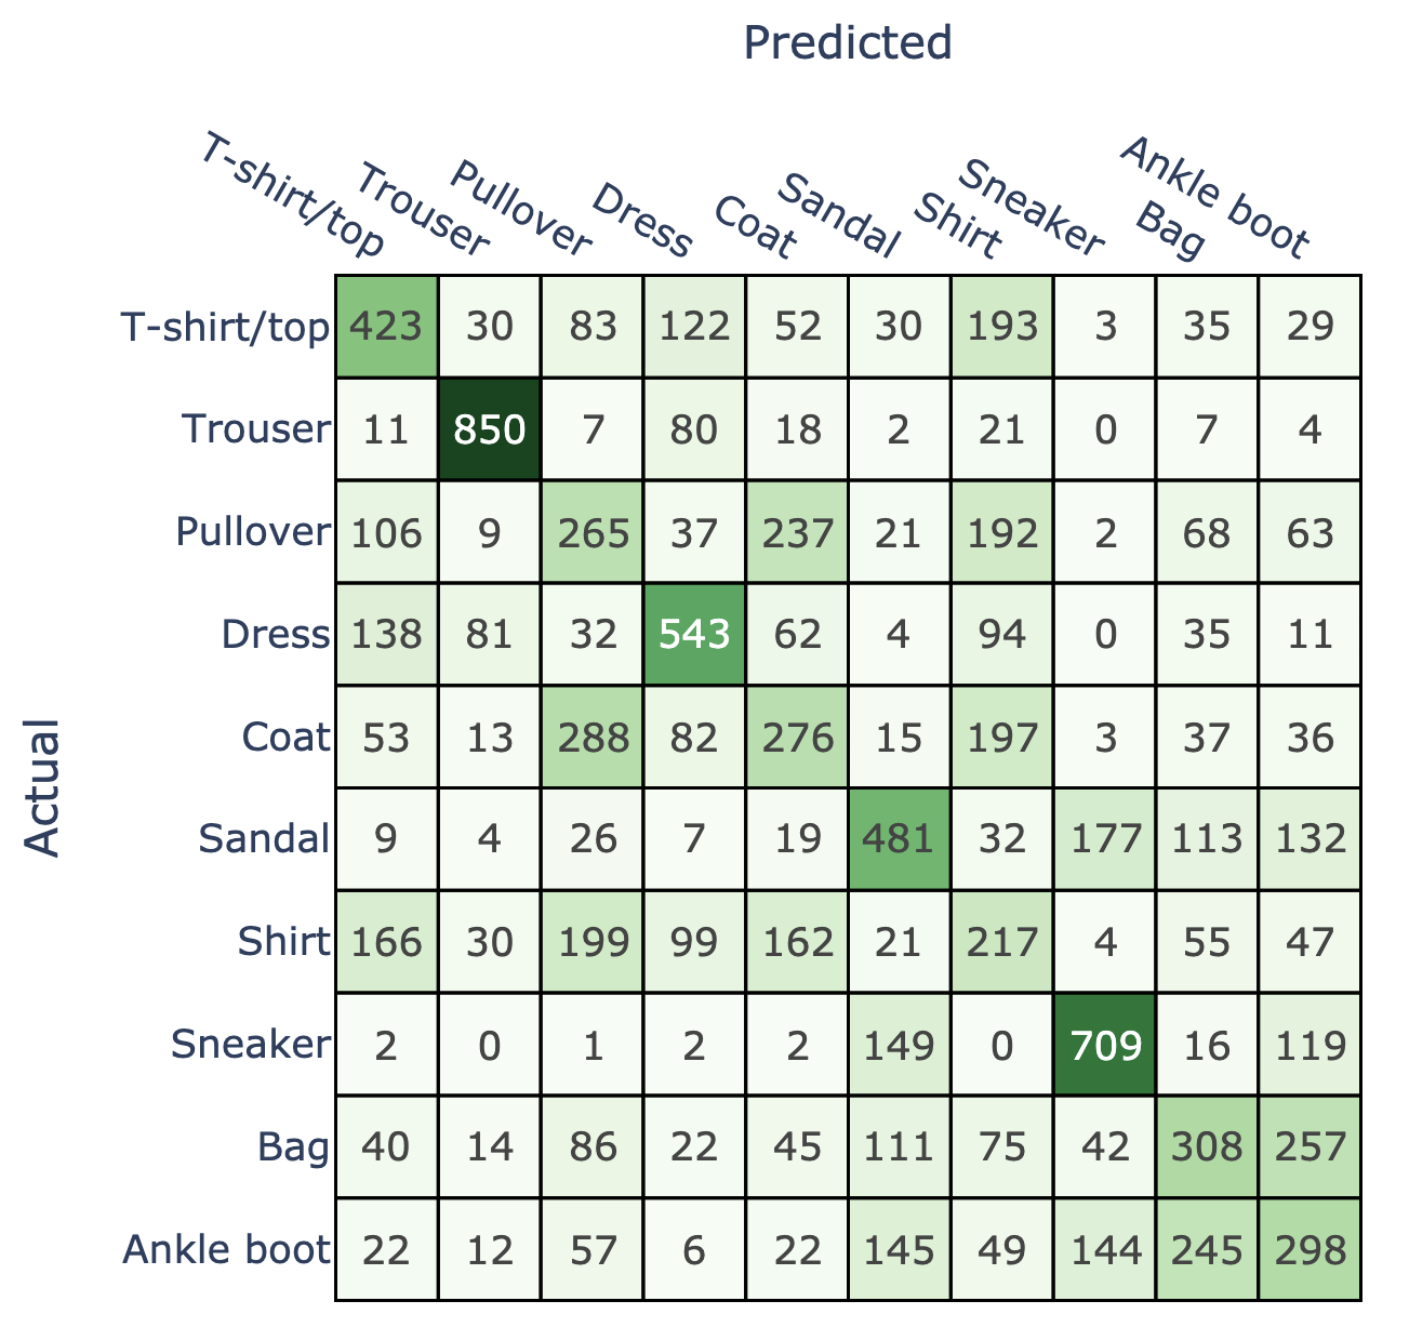
\includegraphics[width=1\linewidth]{images/CM_HybridPipeline_ProbabilisticMapping_CNN.png}
        \subcaption{\footnotesize CNN}
    \end{minipage}
    \caption{\footnotesize Confusion matrices for classification models [Probabilistic Mapping]}
    \label{fig:confusion_matrices_probabilistic}
\end{figure}

% Majority Vote Tables
\begin{table}[H]
    \centering
    \begin{minipage}{0.32\textwidth}
        \centering
        \begin{adjustbox}{max width=1\textwidth}
            \begin{tabular}{|c|c|c|c|}
                \hline
                \textbf{Class} & \textbf{Precision} & \textbf{Recall} & \textbf{F1-Score} \\ \hline
                Ankle boot & NaN & 0.00 & 0.00 \\ 
                Bag & 0.35 & 0.90 & 0.50 \\
                Coat & 0.45 & 0.64 & 0.53 \\ 
                Dress & 0.62 & 0.81 & 0.70 \\ 
                Pullover & NaN & 0.00 & 0.00 \\ 
                Sandal & 0.77 & 0.52 & 0.62 \\ 
                Shirt & 0.29 & 0.40 & 0.34 \\ 
                Sneaker & 0.64 & 0.85 & 0.73 \\ 
                T-shirt/top & 0.82 & 0.41 & 0.55 \\ 
                Trouser & 1.00 & 0.83 & 0.90 \\ \hline
            \end{tabular}
        \end{adjustbox}
        \subcaption{\footnotesize SVC}
    \end{minipage}
    \hfill
    \begin{minipage}{0.32\textwidth}
        \centering
        \begin{adjustbox}{max width=1\textwidth}
            \begin{tabular}{|c|c|c|c|}
                \hline
                \textbf{Class} & \textbf{Precision} & \textbf{Recall} & \textbf{F1-Score} \\ \hline
                Ankle boot & NaN & 0.00 & 0.00 \\ 
                Bag & 0.38 & 0.90 & 0.53 \\ 
                Coat & 0.44 & 0.69 & 0.54 \\ 
                Dress & 0.60 & 0.83 & 0.70 \\ 
                Pullover & NaN & 0.00 & 0.00 \\ 
                Sandal & 0.81 & 0.53 & 0.64 \\ 
                Shirt & 0.29 & 0.37 & 0.33 \\ 
                Sneaker & 0.65 & 0.88 & 0.75 \\ 
                T-shirt/top & 0.80 & 0.45 & 0.58 \\ 
                Trouser & 1.00 & 0.81 & 0.89 \\ \hline
            \end{tabular}
        \end{adjustbox}
        \subcaption{\footnotesize FCNN}
    \end{minipage}
    \hfill
    \begin{minipage}{0.32\textwidth}
        \centering
        \begin{adjustbox}{max width=1\textwidth}
            \begin{tabular}{|c|c|c|c|}
                \hline
                \textbf{Class} & \textbf{Precision} & \textbf{Recall} & \textbf{F1-Score} \\ \hline
                Ankle boot & NaN & 0.00 & 0.00 \\ 
                Bag & 0.35 & 0.88 & 0.50 \\ 
                Coat & 0.46 & 0.63 & 0.53 \\ 
                Dress & 0.60 & 0.81 & 0.69 \\ 
                Pullover & NaN & 0.00 & 0.00 \\ 
                Sandal & 0.77 & 0.54 & 0.64 \\ 
                Shirt & 0.29 & 0.39 & 0.33 \\ 
                Sneaker & 0.64 & 0.88 & 0.74 \\ 
                T-shirt/top & 0.82 & 0.41 & 0.55 \\ 
                Trouser & 1.00 & 0.84 & 0.91 \\ \hline
            \end{tabular}
        \end{adjustbox}
        \subcaption{\footnotesize CNN}
    \end{minipage}
    \caption{\footnotesize Classification reports for models [Majority Mapping]}
    \label{tab:ClassificationReport_Majority}
\end{table}

% Proportional Vote Tables
\begin{table}[H]
    \centering
    \begin{minipage}{0.32\textwidth}
        \centering
        \begin{adjustbox}{max width=1\textwidth}
            \begin{tabular}{|c|c|c|c|}
                \hline
                \textbf{Class} & \textbf{Precision} & \textbf{Recall} & \textbf{F1-Score} \\ \hline
                Ankle boot & 0.31 & 0.30 & 0.31 \\ 
                Bag & 0.32 & 0.32 & 0.32 \\ 
                Coat & 0.32 & 0.31 & 0.31 \\ 
                Dress & 0.53 & 0.52 & 0.52 \\ 
                Pullover & 0.25 & 0.24 & 0.25 \\ 
                Sandal & 0.47 & 0.47 & 0.47 \\ 
                Shirt & 0.21 & 0.22 & 0.21 \\ 
                Sneaker & 0.66 & 0.67 & 0.67 \\ 
                T-shirt/top & 0.45 & 0.45 & 0.45 \\ 
                Trouser & 0.82 & 0.84 & 0.83 \\ \hline
            \end{tabular}
        \end{adjustbox}
        \subcaption{\footnotesize SVC}
    \end{minipage}
    \hfill
    \begin{minipage}{0.32\textwidth}
        \centering
        \begin{adjustbox}{max width=1\textwidth}
            \begin{tabular}{|c|c|c|c|}
            \hline
            \textbf{Class} & \textbf{Precision} & \textbf{Recall} & \textbf{F1-Score} \\ \hline
            Ankle boot & 0.31 & 0.28 & 0.30 \\ 
            Bag & 0.33 & 0.30 & 0.32 \\ 
            Coat & 0.30 & 0.29 & 0.29 \\ 
            Dress & 0.51 & 0.52 & 0.52 \\ 
            Pullover & 0.27 & 0.29 & 0.28 \\ 
            Sandal & 0.48 & 0.45 & 0.46 \\ 
            Shirt & 0.18 & 0.19 & 0.19 \\ 
            Sneaker & 0.65 & 0.70 & 0.68 \\ 
            T-shirt/top & 0.43 & 0.44 & 0.43 \\ 
            Trouser & 0.82 & 0.83 & 0.82 \\ \hline
            \end{tabular}
        \end{adjustbox}
        \subcaption{\footnotesize FCNN}
    \end{minipage}
    \hfill
    \begin{minipage}{0.32\textwidth}
        \centering
        \begin{adjustbox}{max width=1\textwidth}
            \begin{tabular}{|c|c|c|c|}
                \hline
                \textbf{Class} & \textbf{Precision} & \textbf{Recall} & \textbf{F1-Score} \\ \hline
                Ankle boot & 0.30 & 0.30 & 0.30 \\ 
                Bag & 0.34 & 0.31 & 0.32 \\ 
                Coat & 0.31 & 0.28 & 0.29 \\ 
                Dress & 0.54 & 0.54 & 0.54 \\ 
                Pullover & 0.25 & 0.27 & 0.26 \\ 
                Sandal & 0.49 & 0.48 & 0.49 \\ 
                Shirt & 0.20 & 0.22 & 0.21 \\ 
                Sneaker & 0.65 & 0.71 & 0.68 \\ 
                T-shirt/top & 0.44 & 0.42 & 0.43 \\ 
                Trouser & 0.81 & 0.85 & 0.83 \\ \hline
            \end{tabular}
        \end{adjustbox}
        \subcaption{\footnotesize FCNN}
    \end{minipage}
    \caption{\footnotesize Classification reports for models [Probabilistic Mapping]}
    \label{tab:ClassificationReport_Probabilistic}
\end{table}

When adopting the majority labeling approach, we observe NaN values in the precision metric for certain classes. 
This issue arises because the precision computation involves dividing by the total number of predictions for a class, 
and some clothing items are never predicted. Specifically, this affects the ankle boot and pullover classes, which 
consequently exhibit zero recall and F1-scores across all three models (\emph{SVC, FCNN, CNN}). This limitation is mitigated 
by adopting the probabilistic mapping approach, where no class is entirely ignored. While this eliminates NaN values 
and zero metrics, class-level performance does not generally improve. This outcome was expected, since the probabilistic 
approach accounts for minor class contributions within a cluster, which can reduce the overall representativeness of the 
dominant labels. To further analyze this, I retrieved the balanced accuracy from the confusion matrices for both labeling approaches. 
Under the majority mapping approach, the balanced accuracy values resulted 0.54 (\emph{SVC}), 0.55 (\emph{FCNN}) and 0.54 (\emph{CNN}), reflecting modest 
but consistent performance across the models. In contrast, with the probabilistic mapping approach, balanced accuracies decrease
to 0.43 (\emph{SVC}), 0.43 (\emph{FCNN}) and 0.44 (\emph{CNN}).\\[0.2cm]
Among the categories, trousers consistently emerge as the best-classified item across all models and approaches. Remarkably, under the 
majority labeling approach, all models achieve a precision of 1.0 for trousers, meaning that every predicted trouser was correct. This 
result reflects the distinct geometric separation of trousers in the data. Other relatively well-classified categories include T-shirts/tops, 
sandals, and sneakers, with the latter two indicating the models' ability to effectively capture footwear patterns. In contrast, ankle boots 
exhibit poor classification metrics, driven by significant overlap with other classes. Similarly, bags also perform poorly, 
likely due to their observed overlap with ankle boots. Finally, shirts emerge as the most challenging category to classify across all 
models and approaches, with the models consistently struggling to distinguish shirts.\\[0.2cm]
These results, combined with the findings from \Cref{hybrid_model_tuning}, allow us to draw some important conclusions about the 
hybrid pipeline we built. My opinion is that the pipeline effectively captured features and patterns from the unlabeled data during 
the clustering phase. In fact, all the models outperform both the random guessing and the dummy classifier (given the balanced nature 
of the training and test sets, these two almost coincide), which would achieve approximately a 10\% of accuracy. However, there is a notable drop
in performance when transitioning from cluster IDs predictions to the original Fashion-MNIST labels. This is reflected by the 
models’ difficulty in distinguishing between certain categories, which was already clear during the clustering phase 
(recall \Cref{fig:cluster_composition}), where these classes were often overlapped and grouped together. 
The relatively low accuracies (43-44\%) achieved in our mapping step are in contrast to the results typically obtained 
with fully supervised learning on Fashion-MNIST, as we'll see in \Cref{fully_supervised_approach}. These results underscore the inherent 
challenges of our unsupervised-to-supervised approach: while the pipeline demonstrates its ability to learn structure from unlabeled data, 
the limitations in accurately mapping clusters to fine-grained categories highlight the complexity of the task, particularly in cases 
of significant class overlapping.
\newpage